\documentclass[a4paper,rep]{thesisby}

\usepackage[T2A]{fontenc}
\usepackage[utf8]{inputenc}
\usepackage[english, russian]{babel}
\usepackage{lastpage}

\usepackage{amsmath, amssymb, amsfonts}
\usepackage{longtable,array}
\usepackage{fixltx2e}
\usepackage{multirow}

\usepackage{afterpage}

\usepackage{algorithmic}
\usepackage{algorithm}


\usepackage{color}


\emergencystretch=25pt

\newcommand{\abs}[1]{\left\vert#1\right\vert}
\renewcommand{\theequation}{\arabic{equation}}
\renewcommand{\thefigure}{\arabic{figure}}
\renewcommand{\thetable}{\arabic{table}}
\renewcommand{\labelenumii}{\arabic{enumii}}

\newcommand*{\mbb}{\mathbb}
\newcommand*{\mbf}{\mathbf}

\newcommand*{\diff}{\mathop{}\!\mathrm{d}}% Differential
\newcommand*{\pd}{\partial}% Partial differential
\newcommand*{\im}{\ensuremath{\mathrm{i}}}% Imaginary unit
\newcommand*{\e}{\mathop{\mathrm{e}}\nolimits}% The number "e"
\newcommand*{\const}{\ensuremath{\mathrm{const}}}% const
\DeclareMathOperator{\diverg}{div}% Divergence

\newcommand*{\Four}{\mathcal{F}}%{\hat}% Fourier transform
\newcommand*{\Lapl}{\mathcal{L}}%{\tilde}% Laplace transform
\newcommand*{\ctrw}{\mathrm{RW}}
\newcommand*{\dctrw}{\mathrm{DRW}}
\newcommand*{\drwg}{\mathrm{DRWG}}
\newcommand*{\drwb}{\mathrm{DRWB}}
\newcommand*{\te}{\mathrm{TE}}
\newcommand*{\de}{\mathrm{DE}}
\newcommand*{\Gauss}{\mathrm{G}}
\newcommand*{\Bern}{\mathrm{B}}
\newcommand*{\discr}{\mathrm{d}}
\newcommand*{\singul}{\mathrm{s}}
\newcommand*{\regul}{\mathrm{r}}

\newcommand{\Rb}{\mathbb R}
\DeclareMathOperator{\dist}{dist} \DeclareMathOperator{\diam}{diam}

\newcommand{\diffd}[2]{\frac{\partial^2}{\partial #1 \partial #2}}
\newcommand{\sumd}[2]{\sum_{u = #1}^{#2}}
\newcommand{\ceilr}{\lceil r \rceil}
\newcommand{\floor}[1]{\lfloor #1 \rfloor}
\newcommand{\enbrace}[1]{\lb #1 \rb}
\newcommand{\inv}[1]{{#1}^{-1}}
\newcommand{\setdef}[2]{\left\{ #1\ \left|\ #2 \right.\right\}}
\newcommand{\seqz}[2]{\left\{ {#1}_{#2} \right\}_{#2\in\Zb}}
\newcommand{\seq}[1]{ \{ #1 \} }
\newcommand{\half}[1]{\frac{#1}{2}}
\newcommand{\vmod}[1]{\left| #1 \right|}
\newcommand{\Ah}{\hat{A}}
\newcommand{\No}{\textnumero}

\usepackage{minted}
\usepackage{graphicx}
\usepackage{epstopdf}

\textwidth=170mm \textheight=240mm

\makeatletter
\renewcommand\@biblabel[1]{#1 }
\makeatother

\DeclareMathSymbol{\Pi}{\mathalpha}{letters}{"05}

\begin{document}

\graphicspath{{./img/}}

%!TEX root = report.tex
\begin{titlepage}

\begin{center} %\bfseries
{%\fontsize{14.4pt}{4mm}\selectfont
%\large
Министерство образования и науки Российской Федерации\\
%\medskip
Федеральное государственное автономное образовательное учреждение\\
высшего образования\\
<<Санкт-Петербургский политехнический университет Петра Великого>>
}
\end{center}
\vspace{0.5cm}

\hspace{-5mm}
\begin{tabular}{lcr}
{
	\begin{tabular}[t]{l}
		УДК\\
		\No{} \\
		Инв. \No{} \\
	\end{tabular}
} & \hspace{40mm} & {
	\begin{tabular}[t]{l}
		У Т В Е Р Ж Д А Ю \\
		Зав. НИЛ <<Математическая биология\\
		и биоинформатика>>, ИПММ\\
		ФГАОУ ВО <<СПбПУ>>,\\
		д.б.н. \\
		\underline{\hspace{4cm}} М. Г. Самсонова\\
		<<\underline{\hspace{1cm}}>> \underline{\hspace{3cm}} 2016 г.
	\end{tabular}
}\\
\end{tabular}
\vspace{2cm}



\begin{center}
{%\bfseries
%\large
ОТЧЕТ\\
ПО КУРСОВОЙ РАБОТЕ\\
\vspace{3mm}
по предмету:\\
<<Системная биология>>\\
}
\end{center}

\vspace{1.5cm}


\hspace{15mm}
\begin{tabular}{ll}
{
	\hspace{60mm}
}&{
	\begin{tabular}[t]{l}
		Выполнил студент гр. \No{63601/4}\\
		{}\\
		\underline{\hspace{2cm}} Д. В. Яковлев\\
		<<\underline{\hspace{1cm}}>> \underline{\hspace{3cm}} 2016 г.
	\end{tabular}
}\\
{
	{}
}&{
}\\
{
	{}
}&{
	\begin{tabular}[t]{l}
		Руководитель НИР, к.ф.-м.н. \qquad\\
		{}\\
		\underline{\hspace{2cm}} В.В. Гурский \\
		<<\underline{\hspace{1cm}}>> \underline{\hspace{3cm}} 2016 г.
	\end{tabular}
}\\
\end{tabular}
\vspace{20mm}

\begin{center}
 %\large
 Санкт-Петербург 2016
\end{center}

\end{titlepage}


\newpage
\tableofcontents


\newpage
%!TEX root = report.tex

\section{Введение}

В данной работе предлагается рассмотреть систему репрессилатора  - три системы транскрипционных репрессора, которые не являются частью
каких-либо естественных биологических часов, чтобы построить колебательный сети. В роли программного обеспечения для анализа системы будет
использоваться пакет COPASI.

COPASI - это программа с открытым исходным кодом для создания и решения математических моделей биологических процессов,
таких как метаболические сети, сигнальные пути клеток, регуляторные сети, инфекционные заболевания и многое другое.

Цель работы - знакомство с пакетом COPASI на примере системы репрессилатора.

\section{Система}
Система состоит из 12 биохимических реакций и 7 реагентов.
Реагенты:
\begin{itemize}
  \item X, PX - мРНК и протеин гена LacI
  \item Y, PY - мРНК и протеин гена tetR
  \item Z, PZ - мРНК и протеин гена Cl
\end{itemize}

Реакции системы представлены на рисунке \ref{ris:reactions}.
\begin{figure}[!h]
\center{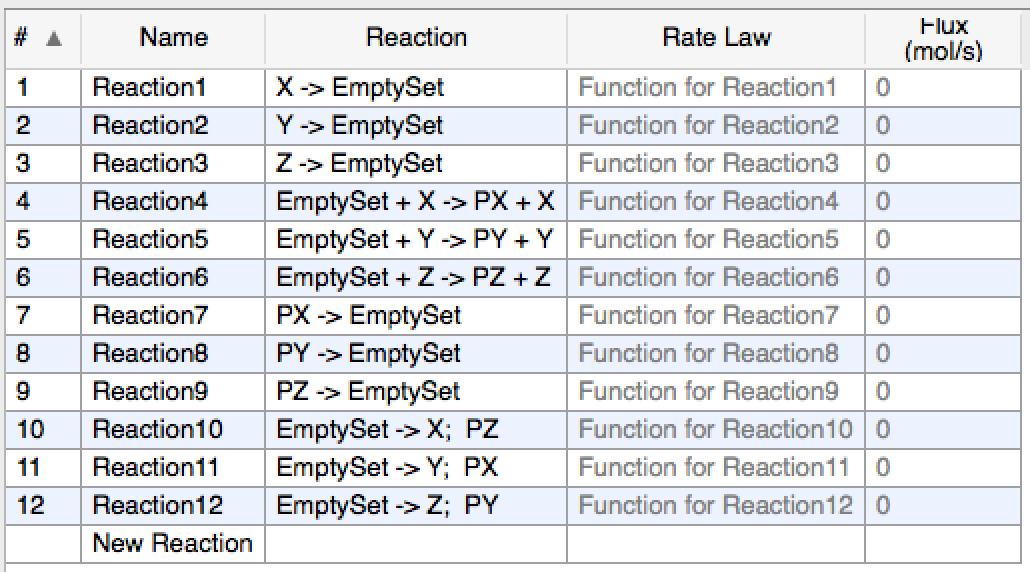
\includegraphics[width=1\linewidth,height=8cm]{reactions}}
\caption{Биохимические реакции системы репрессилатора}
\label{ris:reactions}
\end{figure}

C системой дифференциальных уравнений для нашей системы можно познакомиться на рисунке \ref{ris:equations}.
\begin{figure}[!h]
\center{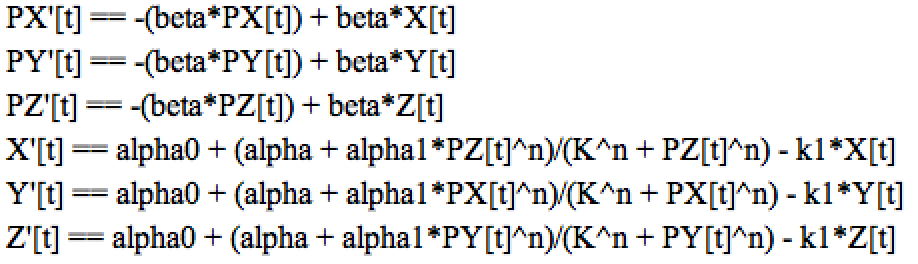
\includegraphics[width=1\linewidth]{equations}}
\caption{Дифференциальные уравнения системы репрессилатора}
\label{ris:equations}
\end{figure}

\section{Анализ динамики системы}
Первоначально исследуем поведение системы на промежутке 1 секунда с размером интервала 0.01 секунда (Рис. \ref{ris:plot1}). В данном случаем
нам сложно что-то утверждать о поведении концентрации tetR и Cl.

\begin{figure}[!h]
\center{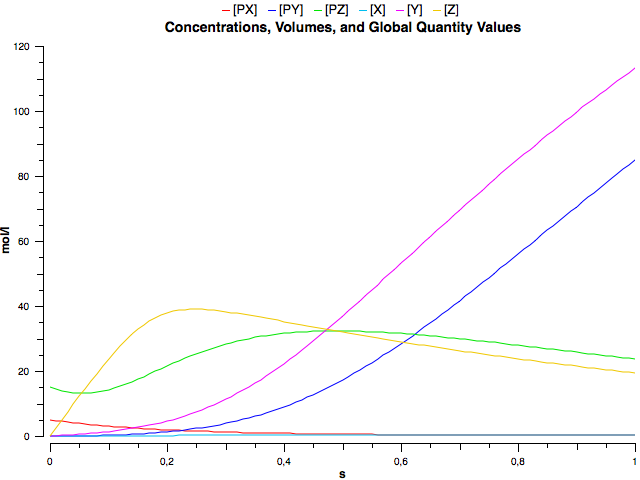
\includegraphics[width=1\linewidth,height=9cm]{plot1}}
\caption{Динамика поведения системы на промежутке 1 секунда}
\label{ris:plot1}
\end{figure}

Увеличим временной промежуток до 10 секунд (Рис. \ref{ris:plot2}). Теперь мы можем сравнивать между собой кривые. На графике отчётливо видно,
что мРНК и протеин для одного гена изменяются одинаково.

\begin{figure}[!h]
\center{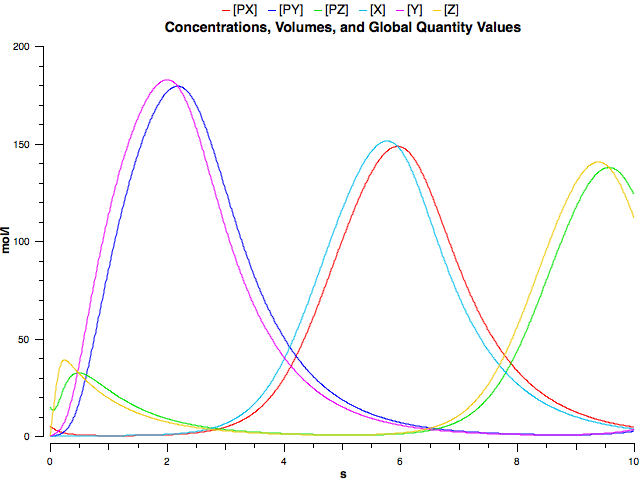
\includegraphics[width=1\linewidth]{plot2}}
\caption{Динамика поведения системы на промежутке 10 секунд}
\label{ris:plot2}
\end{figure}

С увеличением временного промежутка до 50 секунд можно утверждать закономерности изменения концентраций мРНК и протеина(Рис. \ref{ris:plot3}).
То есть сначала вырабатывается мРНК и протеин tetR из Cl, далее из них получается мРНК и протеин LacI и в конце имеем мРНК и протеин Cl
после чего процесс повторяется.

\begin{figure}[!h]
\center{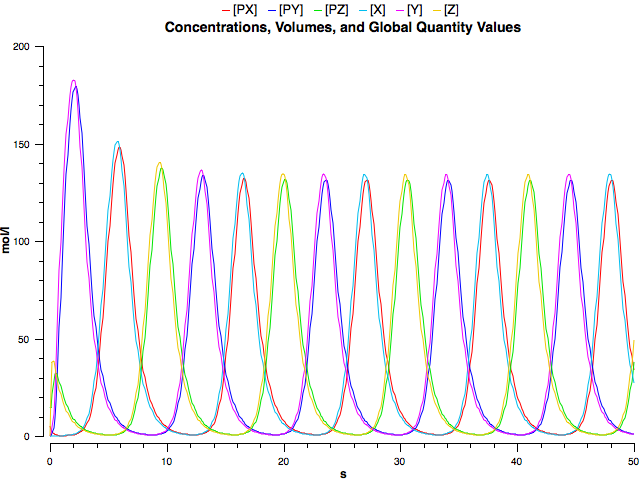
\includegraphics[width=1\linewidth]{plot3}}
\caption{Динамика поведения системы на промежутке 50 секунд}
\label{ris:plot3}
\end{figure}

\newpage
\section{Анализ состояния равновесия системы}
Пакет COPASI предлагает три подхода к поиску состояния равновесия:
\begin{enumerate}
  \item Метод Ньютона
  \begin{itemize}
    \item Быстрый
    \item Не гарантируется сходимость
  \end{itemize}
  \item Метод интегрирования
  \begin{itemize}
    \item Медленнее
    \item Гарантируется сходимость
  \end{itemize}
  \item Метод обратного интегрирования
  \begin{itemize}
    \item Используется в крайне редких случаях
  \end{itemize}
\end{enumerate}

С помощью метода Ньютона обнаружить состояние равновесие не удалось (Рис. \ref{ris:newton}).

\begin{figure}[!h]
\center{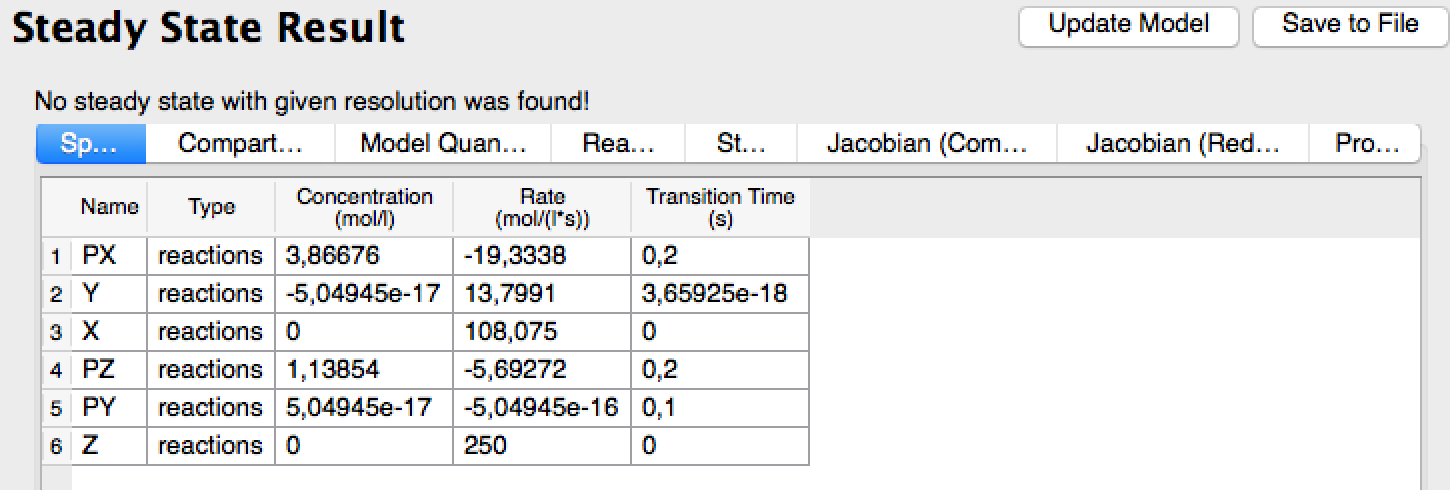
\includegraphics[width=1\linewidth]{newton}}
\caption{Результат поиска состояния равновесия с помощью метода Ньютона}
\label{ris:newton}
\end{figure}

Однако с помощью метода интегрирования удалось найти состояние равновесия (Рис. \ref{ris:int}).

\begin{figure}[!h]
\center{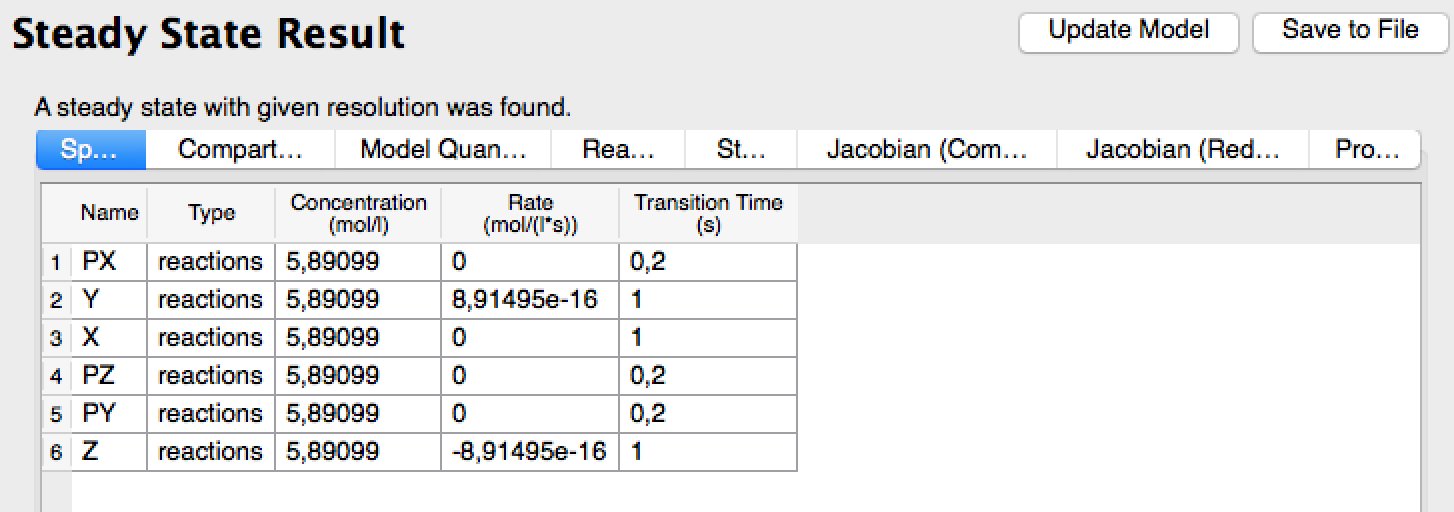
\includegraphics[width=1\linewidth]{int}}
\caption{Результат поиска состояния равновесия с интегрирования}
\label{ris:int}
\end{figure}

Теперь зная состояние равновесия, обновим модель и посмотрим динамику системы.
На рисунке \ref{ris:steady} можем наблюдать, что система находится в состоянии равновесия.

\begin{figure}[!h]
\center{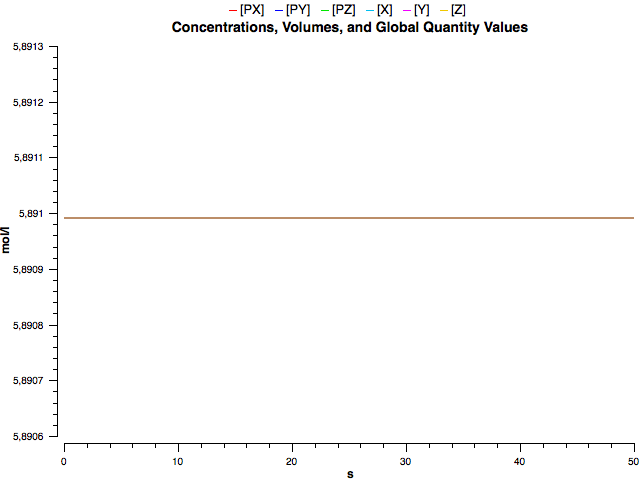
\includegraphics[width=1\linewidth]{steady}}
\caption{Динамика системы в состоянии равновесия}
\label{ris:steady}
\end{figure}

\section{Анализ параметров системы}
Наша система имеет параметры - beta, alpha0, alpha1, K, k1, n. Посмотрим, как меняется поток реакции 12 в состоянии равновесия
при изменении параметра n. Как видно по рисунку \ref{ris:scan} никак не изменяется поток в зависимости от n.
К сожалению, попытки получить более красивые графики не увенчались успехом (проверялись другие параметры в остальных реакциях).

\begin{figure}[!h]
\center{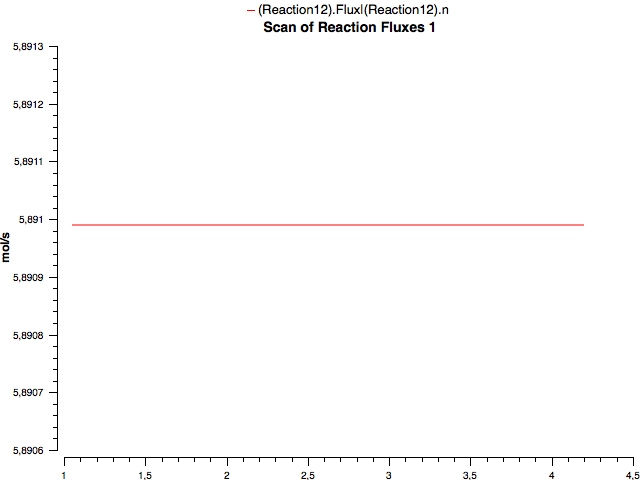
\includegraphics[width=1\linewidth]{scan}}
\caption{Изменение потока в зависимости от параметра n}
\label{ris:scan}
\end{figure}

\section{Выводы}
Пакет COPASI предоставляет нам следующие возможности:
\begin{itemize}
  \item Работа с системами биохимических реакций. Возможность создавать новые, записывать в виде дифференциальных уравнений реакции и т.д.
  \item Анализ динамики системы на определённом временном промежутке с заданным интервалом
  \item Поиск состояния равновесия
  \item Анализ параметров системы
\end{itemize}



\end{document}
